\subsection{Scalar Fields > Arithmetic}
\label{subsection:scalarFieldDiff}

\index{champ scalaire}
\index{diff�rence}

\begin{figure}[!h]
\begin{center}
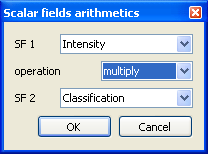
\includegraphics[width=0.3\textwidth]{Partie3_Fonctions/sfArtithmetic.png}
\caption{\label{fig:sfArtithmetic}Interface de la m�thode << Scalar Fields > Arithmetic >>}
\end{center}
\end{figure}

Cet outil permet d'effectuer des op�rations �l�mentaires (addition, soustraction, multiplication et division) entre des champs scalaires d'un m�me nuage.\\
\par
Pour appeler cette m�thode, un seul nuage doit �tre s�lectionn�. L'utilisateur doit alors choisir un champ scalaire $A$ et un champ scalaire $B$ ainsi qu'un type op�ration (voir figure~\ref{fig:sfArtithmetic}). Un champ scalaire $champ_{C} = champ_{A} op champ_{B}$ sera alors cr��.\\
\par
Remarque : le champ scalaire cr�� ($C$) est par d�faut sign�, m�me si les champs $A$ et $B$ sont non sign�s. Si cela est n�cessaire, l'utilisateur peut manuellement sp�cifier que ce champ scalaire est non sign� (voir section~\ref{Champs-scalaires} - case � cocher \emph{Postive}).

